\chapter{Introducción}\label{cap.introduccion}

Debido al crecimiento en la población se ha visto incrementada la cantidad de vehículos que se encuentran en circulación. Este incremento en la densidad de vehículos ha afectado en el tráfico y en la contaminación. Por ello se han ido buscando formas de mejorar la seguridad vial y el rendimiento en las carreteras. En este punto es donde intervienen las nuevas tecnologías, las cuales son capaces de ofrecernos mucha información para poder mejorar el tráfico. Esta aplicación de sistemas avanzados de información y comunicación a las infraestructuras de transporte y a los vehículos para mejorar la seguridad vial, la eficiencia y el rendimiento de las carreteras se denomina Sistemas inteligentes de transporte (SIT). Este area está en continuo desarrollo y con ello se pretende dotar a los vehículos de inteligencia para aportarnos información con la cual mejorar nuestra seguridad y monitorizar las redes de transporte para detectar posibles incidencias y mejorar el tráfico.


\begin{figure}[H]
  \begin{center}
    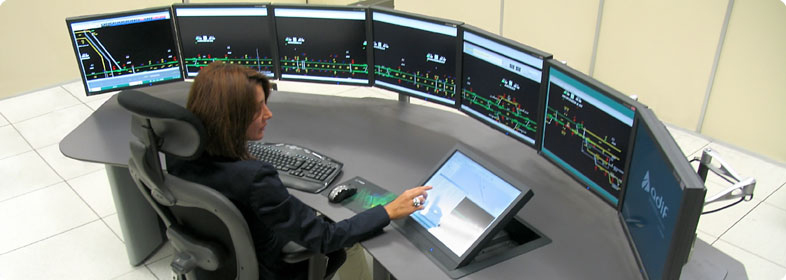
\includegraphics[width=0.6\textwidth]{figures/Introduccion/Indra.jpg}
		\caption{Centro de monitorización de tráfico}
		\label{fig.monitorizacion}
		\end{center}
\end{figure}

Los sistemas tradicionales de monitorización ofrecen una información muy limitada, pues normalmente es un humano el que analiza toda la información que le aportan las cámaras y con ello toma las decisiones. Gracias a los últimos avances en visión artificial muchas de las tareas que realizaba el humano se han podido automatizar. Con la visión artificial somos capaces de procesar todas las imágenes que recogen las cámaras y extraer información de ellas, como por ejemplo la cantidad de tráfico que hay, las condiciones meteorológicas que tenemos, la existencia de incidencias, etc.

Los principales sectores de los SIT son:
\begin{enumerate}
    \item Gestión avanzada del transporte
    \item Gestión avanzada del transporte público
    \item Sistemas de cobro automático
\end{enumerate}

El primer sector hace referencia a la gestión de carreteras a nivel global. Sus funciones principales son agilizar el tráfico, mejorar la movilidad, optimizar el uso de las infraestructuras y mejorar la seguridad de las redes de transporte. Para conseguir todo esto se emplea como sensor principal las cámaras. Con dichas cámaras se obtienen imágenes en todo momento, las cuales son procesadas y analizadas por seres humanos o automáticamente mediante algoritmos de visión artificial.  

El segundo sector tiene el mismo fin que el primer sector pero limitado a sistemas de transporte público. Entre sus funciones se encuentra gestionar de forma eficaz y optimizada las redes de transporte público, e informar  a los ciudadanos acerca de las distintas alternativas de transporte disponibles así como sus horarios o sus posibles incidencias en tiempo real. Este sector también se encarga de todo lo referente a los sistemas de cobro y el manejo de billetes en el transporte. Su objetivo es facilitar la integración y unificación de los sistemas de cobro para facilitar la creación de billetes multimodales y tarjetas de transporte subvencionadas por el estado.

El último sector (sector de cobro automático) se encarga de todos los sistema electrónicos de gestión de cuotas. La gestión de cobros automáticos en autopista con sistemas de telepeaje se basa en el empleo de sistemas inalámbricos de comunicación entre el sistema de gestión de cobro y el vehículo. En estos sistemas el vehículo debe disponer de un dispositivo, el cual permite identificarlos de manera segura y gestionar su cuota sin necesidad de que el vehículo se detenga en el telepeaje. Con esto se consigue reducir el atasco en los peajes.

A parte de la división a nivel sectorial de los SIT explicada, existe una división a nivel de aplicaciones. Esto puede verse en la Figura \ref{fig.division_SIT}.

\begin{figure}[H]
  \begin{center}
    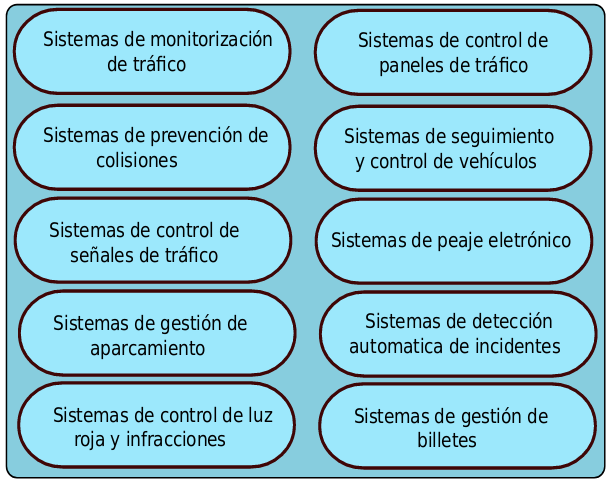
\includegraphics[width=0.6\textwidth]{figures/Introduccion/Division_SIT.png}
		\caption{División del sector SIT a nivel de aplicación}
		\label{fig.division_SIT}
		\end{center}
\end{figure}

\section{Cámaras en tecnologías automóviles y su entorno}

Si pensamos en una ciudad inteligente lo primero que nos viene a la cabeza son cámaras. Actualmente las cámaras se emplean en muchos ámbitos debido a la gran calidad que ofrecen, lo económicas que son y su reducido tamaño. Esto hace que sean uno de los mejores sensores de los que disponemos. Con las imágenes que nos ofrecen las cámaras necesitamos implementar algoritmos que sean capaces de procesarlas, extraer información y analizarla. Una de las aplicaciones pioneras donde la visión artificial ha demostrado ser una solución práctica frente a otras alternativas es la detección de matrículas. Este caso en concreto se usa en muchas puertas de acceso a aparcamientos, pues ha demostrado que tiene una gran fiabilidad. Además el hecho de encontrarse en puertas de acceso a aparcamientos hace que se trata de escenarios muy controlados, pues conocemos la iluminación del lugar, la posición que toman los vehículos, etc. Esto es una gran ventaja, pues nos aporta información adicional facilitándonos la identificación de las matrículas.

\begin{figure}[H]
  \begin{center}
    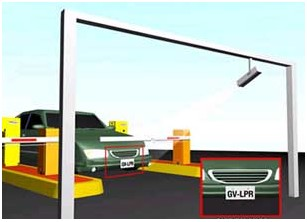
\includegraphics[width=0.6\textwidth]{figures/Introduccion/reconocimiento_matriculas.jpeg}
		\caption{Sistema de reconocimiento automático de matrículas}
		\label{fig.reconocimiento_matriculas}
		\end{center}
\end{figure}

Otra aplicación de las cámaras son los radares de tramo. En este caso se pretende calcular la velocidad media de cada vehículo haciendo uso del reconocimiento de matrículas. Las cámaras suelen situarse en los extremos de un túnel, ya que la trayectoria del vehículo está bajo control.

\begin{figure}[H]
  \begin{center}
    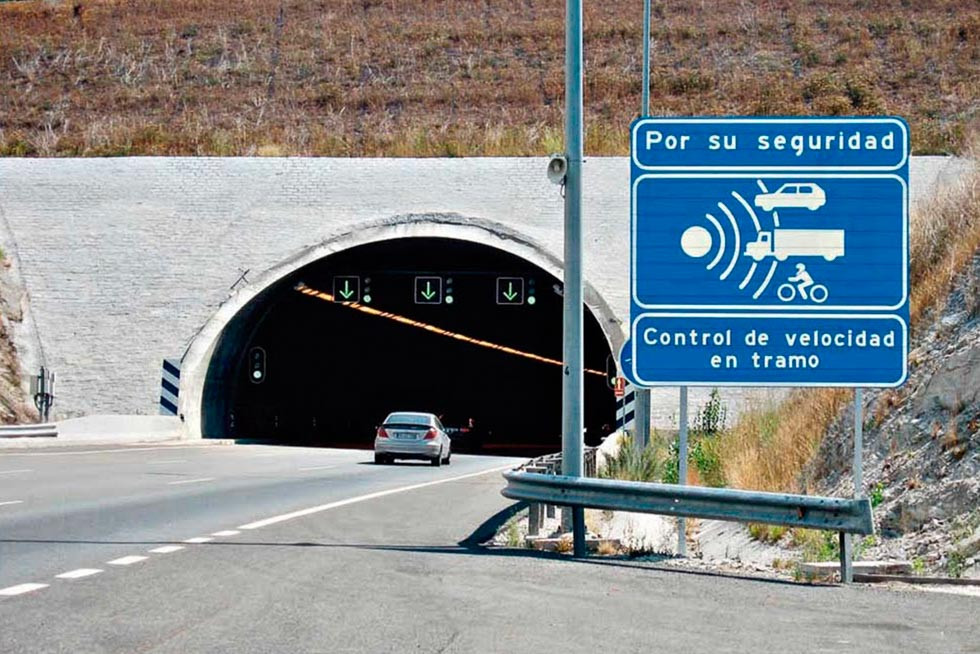
\includegraphics[width=0.6\textwidth]{figures/Introduccion/radartramo.jpg}
		\caption{Radar de tramo basado en reconocimiento de matrículas}
		\label{fig.radartramo}
		\end{center}
\end{figure}

Otro campo en el que cada vez tienen mayor relevancia las cámaras es en seguridad vial. Hoy en día hay varios modelos de coches capaces de detectar señales de tráfico de manera automática. De esta forma el vehículo puede avisar al conductor del exceso de velocidad, de la dirección de la próxima curva, etc. Este tipo de sistemas se encuentran incorporados en vehículos de marcas comerciales como BMW 7-series, Ford Focus, Toyota, Opel Insignia, etc.

\begin{figure}[H]
  \begin{center}
    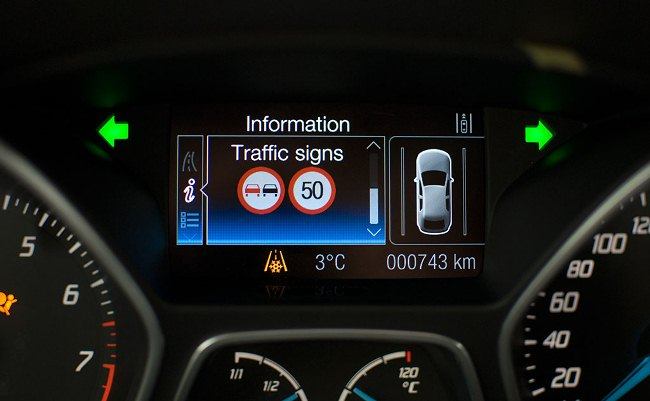
\includegraphics[width=0.6\textwidth]{figures/Introduccion/deteccion_senales.jpg}
		\caption{Sistema de ayuda a bordo del vehículo}
		\label{fig.deteccion_senales}
		\end{center}
\end{figure}

Disponer de cámaras en los vehículos ha hecho posible aumentar la seguridad, pues nos aportan mucha información. Actualmente existen modelos de vehículos que nos avisan de la presencia de peatones e incluso poseen mecanismos de frenado automático evitando posibles atropellos.

Una aplicación de las cámaras muy presente en los vehículos es el asistente para el aparcamiento.  En esta aplicación en concreto, las cámaras pueden aportar imágenes acerca de los alrededores de nuestro vehículo ,ofreciéndonos información acerca de como debemos aparcar, e incluso forman parte de  sistemas multisensoriales para aparcar automáticamente.

\begin{figure}[H]
  \begin{center}
    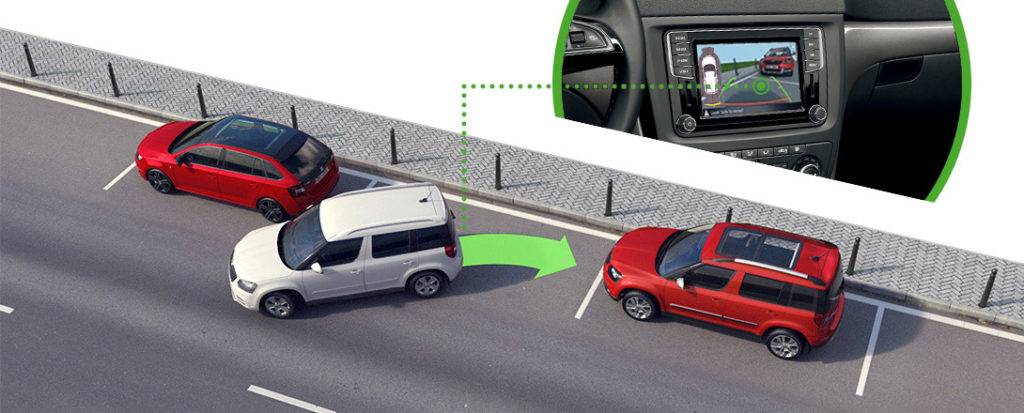
\includegraphics[width=0.6\textwidth]{figures/Introduccion/aparcamiento_automatico.jpg}
		\caption{Aparcamiento automático}
		\label{fig.aparcamiento_automatico}
		\end{center}
\end{figure}

Un ejemplo de asistencia en el aparcamiento es el sistema de ojo de pájaro de Nissan. Dicho sistema ofrece una vista aérea simulada de la escena del aparcamiento. En ella se incluye el vehículo y sus alrededores, ofreciéndole al conductor gran información acerca de la situación. Con lo que podrá realizar la maniobra de forma más sencilla y segura. Para conseguir esto, el vehículo dispone de 4 cámaras, las cuales emplea para generar la simulación. A parte de esta simulación, el conductor puede usar la cámara trasera para obtener más detalles de la escena.

\begin{figure}[H]
  \begin{center}
    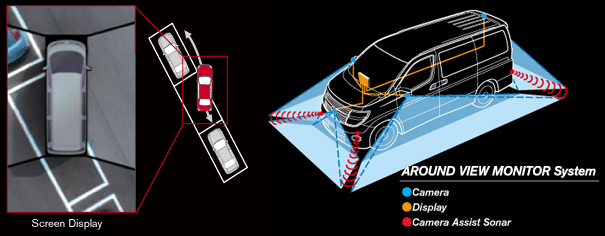
\includegraphics[width=0.6\textwidth]{figures/Introduccion/nissan.jpg}
		\caption{Sistema de visión de ojo de pájaro para asistencia en el aparcamiento}
		\label{fig.nissan}
		\end{center}
\end{figure}

BMW tiene un sistema un poco más evolucionado, pues  a parte del sistema de Nissan, posee una cámara trasera con sensores que miden las distancias con los obstáculos. En la imagen que ofrece proyecta una serie de líneas que ayudan en la orientación del vehículo durante la maniobra de aparcamiento. Estas imágenes son enriquecidas con marcas 3D que se basan en un código de color para marcar la distancia con los obstáculos. Además de todo esto, el sistema proporciona al conductor un mapa del vehículo y los obstáculos que le rodean en todo momento.

\begin{figure}[H]
  \begin{center}
    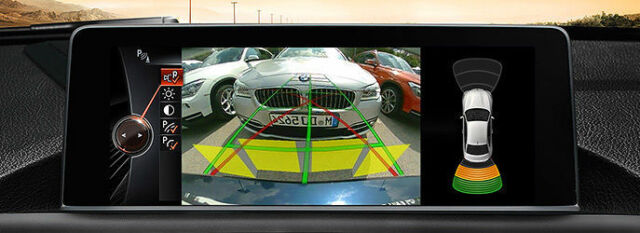
\includegraphics[width=0.6\textwidth]{figures/Introduccion/bmw.jpg}
		\caption{ Cámara trasera de BMW para asistencia en el aparcamiento}
		\label{fig.bmw}
		\end{center}
\end{figure}

Hoy en día uno de los campos en continua evolución es el de los coches autónomos, pues cada día hay más empresas interesadas en ello. Pero este tema no es tan actual, ya que en 1950 ya se trataba de crear coches autónomos. Y desde entonces se han conseguido continuos avances en su mayor medida destinados a aportar a los vehículos sistemas para navegar de forma autónoma.

Los coches autónomos disponen de un radar en la parte frontal para detectar vehículos próximos. Este sensor se emplea para mantener la distancia de seguridad con el vehículo que se encuentra delante y para posibles frenadas de emergencia si fueran necesarias. En las ruedas traseras tienen un sensor ultrasonido capaz de detectar obstáculos muy cercanos al vehículo, permitiendo con ello realizar maniobras muy precisas. Este sensor es muy práctico en el aparcamiento autónomo, pues ofrece información muy precisa en todo momento acerca de los obstáculos que se encuentren en la parte trasera. En la parte superior del vehículo se dispone de una antena GPS, una cámara Lidar y una cámara frontal. La antena GPS permite que el vehículo pueda localizarse con gran precisión en exteriores. La cámara Lidar (Light detection and ranging) realiza un barrido continuo de 360º para construir un mapa 3D de los alrededores del vehículo. La cámara frontal analiza todo lo que el vehículo tenga en frente, como por ejemplo señales de tráfico, peatones, otros vehículos, etc. A parte de todo lo comentado por supuesto contienen un ordenador a bordo que analiza la información captada por todos los sensores y en función a ella toma las decisiones que correspondan.Todos estos sensores pueden verse en la Figura \ref{fig.coche_autonomo}.

\begin{figure}[H]
  \begin{center}
    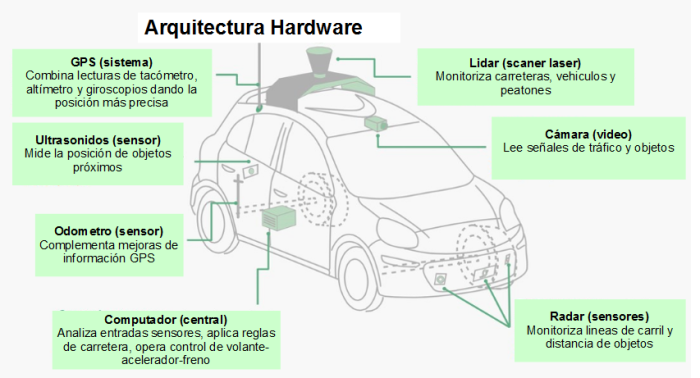
\includegraphics[width=0.6\textwidth]{figures/Introduccion/coche_autonomo.png}
		\caption{ Sensores en vehículos autónomos}
		\label{fig.coche_autonomo}
		\end{center}
\end{figure}

Si hablamos de conducción autónoma no nos podemos olvidar de mencionar al DARPA Grand Challenge. Se trata de una competición donde vehículos autónomos tratan de completar un circuito en el desierto en un tiempo determinado. En ella puede inscribirse cualquier entidad ya sea privada o pública. De hecho se pueden encontrar participando desde universidades hasta empresas privadas. Esta competición fue creada por la agencia de investigación DARPA con el objetivo de incentivar la creación y el desarrollo de vehículos autónomos capaces de  llevar a cabo misiones preplanificadas. Con ello se pretende poder emplear esta tecnología en misiones de exploración así como para aplicaciones militares.


La agencia DARPA también organiza la competición DARPA Urban Challenge. Esta competición tiene la misma dinámica que la mencionada anteriormente pero se desarrolla en un entorno urbano, el cual consta de 96km los cuales deben completarse en menos de 6 horas. Durante el trayecto los vehículos tienen que interactuar con otros vehículos autónomos o vehículos ocupados por conductores profesionales. En este caso la competición es más compleja que la comentada anteriormente, pues durante el circuito si tenemos señales de tráfico, las cuales deben respetarse. Con esto se pretende desarrollar vehículos que se puedan emplear en la vida cotidiana.

\begin{figure}[H]
  \begin{center}
    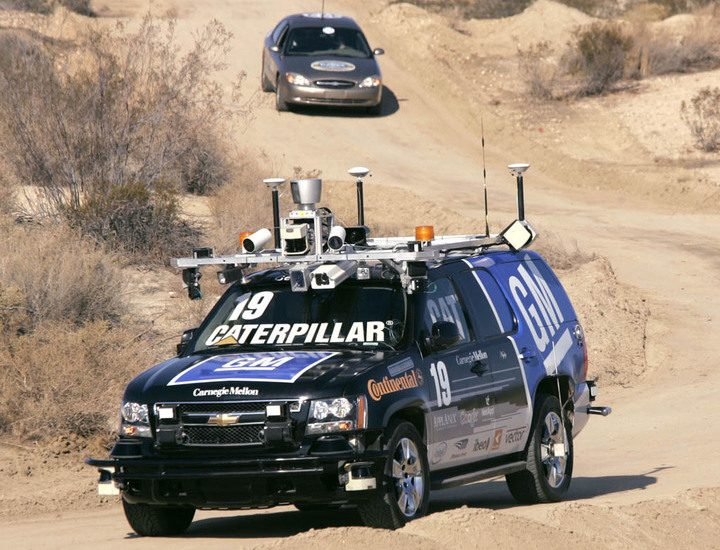
\includegraphics[width=0.6\textwidth]{figures/Introduccion/darpa.jpg}
		\caption{ Vehículo autónomo participante en el \textit{DARPA Grand Challenge}}
		\label{fig.darpa}
		\end{center}
\end{figure}


A pesar de todas las empresas implicadas en este desarrollo de vehículos autónomos la más famosa en este campo es Google. La división de coches autónomos de Google, conocida como Waymo, lleva varios años probando sus vehículos en situaciones reales. La única condición que tienen es que haya un conductor capaz de intervenir en caso de ser necesario ante una emergencia o posibles percances. Estos vehículos ofrecen continuamente información acerca de todo lo que les rodea, ya sea acerca de los peatones que hay, de los vehículos que les rodean, de las señales de tráfico, etc. Pues todo esto es por supuesto necesario para poder realizar una condución totalmente autónoma. El coche de Google además posee un sensor Lidar capaz de alcanzar una distancia máxima de 200 metros.

\begin{figure}[H]
  \begin{center}
    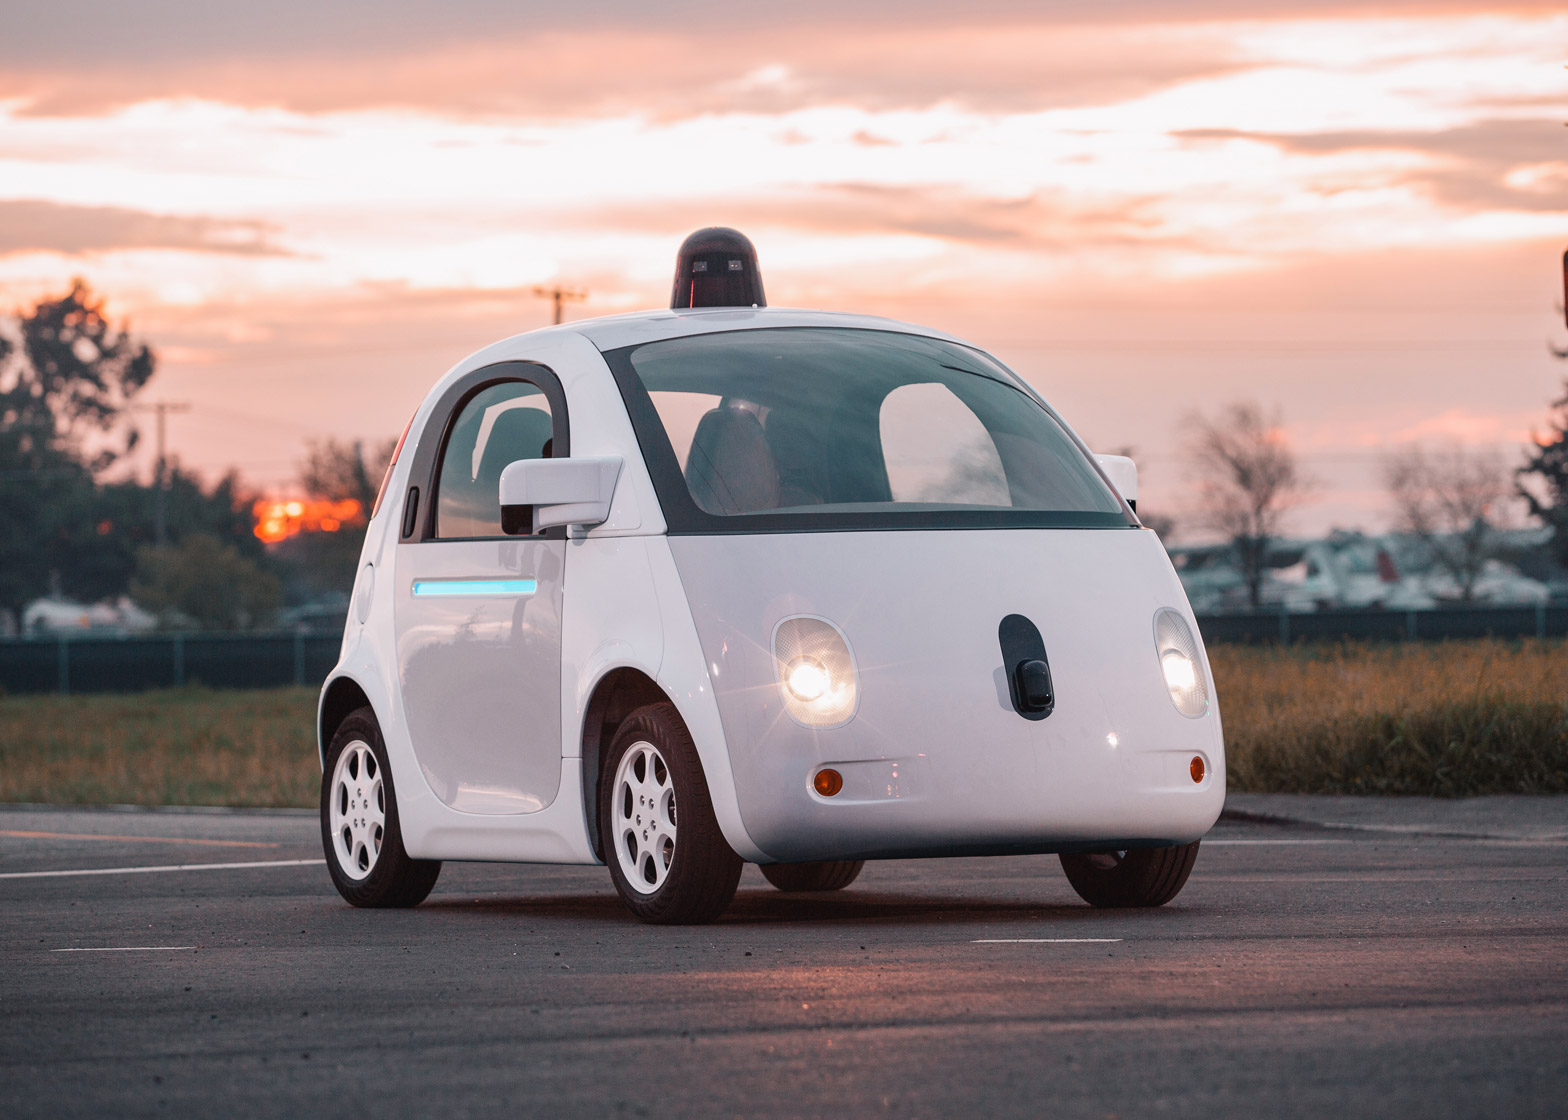
\includegraphics[width=0.6\textwidth]{figures/Introduccion/google_car.jpg}
		\caption{ Vehículo autónomo de Google}
		\label{fig.google_car}
		\end{center}
\end{figure}

Otra de las empresas más importantes en el desarrollo de vehículos autónomos es Tesla. Actualmente Tesla está comercializando el modelo S ,el modelo 3, el modelo X y el modelo Y, los cuales disponen de un piloto automático para activar la conducción autónoma, pero necesita una supervisión activa del conductor por si necesitará tomar el control en cualquier emergencia. A pesar de esto los nuevos vehículos Tesla tienen el hardware que será necesario en el futuro para una conducción completamente automática en la mayoría de situaciones. Pero la ley aún prohíbe dicha conducción autónoma sin supervisión del conductor. Además de esto poseen un asistente de aparcamiento, la posibilidad de aparcar automáticamente, un radar de largo alcance capaz de detectar peatones y obstáculos con una gran antelación, un sonar ultrasónico envolvente que monitoriza el coche desde todos los ángulos, cámaras que detectan señales de tráfico, peatones y otros vehículos, y un sistema de navegación GPS.

\begin{figure}[H]
  \begin{center}
    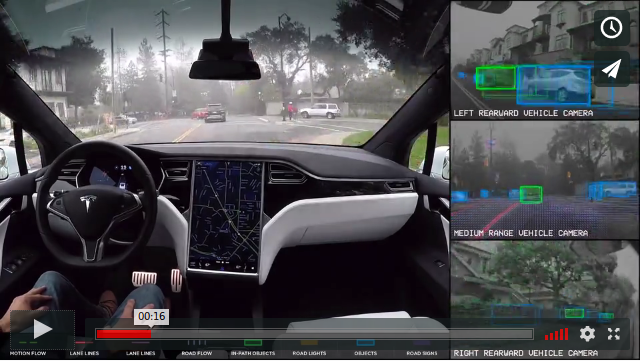
\includegraphics[width=0.6\textwidth]{figures/Introduccion/tesla.png}
		\caption{ Vehículo autónomo de Tesla}
		\label{fig.tesla}
		\end{center}
\end{figure}

\section{Las cámaras como sensor de tráfico}

En comparación con otras disciplinas, la aplicación de la visión computacional en el análisis del tráfico es un campo de estudio muy joven. Las primeras aplicaciones de este tipo fueron presentadas por Onoe  M.,  Ohba  K.~\cite{digital_analisis} y Hilbert~\cite{wide_area}. Pero hasta la década de los 80 no hubo una actividad constante de publicaciones. En este periodo ya podemos encontrar referencias a aplicaciones basadas en visión artificial y orientadas al análisis del tráfico de vehículos. Por ejemplo Hoose, N~\cite{queue_detection} en 1989 presentó una técnica para calcular de manera automática la longitud de la cola formada por vehículos parados o circulando a una velocidad muy reducida. Ese año J.M Blosseville, C. Krafft, F. Lenior,V. Motyka, S. Beucher~\cite{traffic_measurement} presentaron el sistema TITAN, el cual es capaz de analizar escenas de entre 100 hasta 300 metros de longitud, día y noche. Con ello extrae parámetros tales como el flujo de vehículos, la velocidad y la longitud de la cola en atascos, todo esto con una velocidad de procesamiento de 4 imágenes por segundo. Las características más importantes de este trabajo son las luces de noche y los techos, capós y sombras frontales de día. 

En 1989 Versavel, J. ;Lemaire, F. ; Van der Stede, D.~\cite{computer_aided} también presentó el sistema CCATS, el cual obtiene parámetros del tráfico como la ocupación de los carriles, el número de vehículos y la velocidad media de estos.

Además puede detectar anomalías en el flujo de vehículos como atascos o largas colas y alertar acerca de ello. Para mejorar el tráfico este sistema fue instalado en Bélgica.

Hasta finales de los 80 los trabajos se centraron en un macro análisis del tráfico para extraer datos relativamente simples. A partir de los 90 esto va a cambiar pues aumentará la investigación en este sector y se empezarán a realizar análisis más detallados de las escenas basándose en las características visuales de los vehículos. Es entonces cuando se empieza a usar plantillas 3D para la clasificación y seguimiento de vehículos. Baker, K.D Sullivan, G.D.~\cite{performance_assessment} se dedicaron a analizar la viabilidad del seguimiento del tráfico basándose en modelos 3D. Para este seguimiento de tráfico han empleado reconocimiento y estimación de posición en secuencias de imágenes. En esa época el reconocimiento y estimación de posición estaba pensado para una sola imagen , por lo que fueron pioneros al aplicarlo en secuencias de imágenes. En su trabajo disponían de información a priori acerca de la escena 3D, la cual obtenían mediante una cámara calibrada. A pesar de no funcionar en tiempo real este trabajo fue el que abrió las puertas hacia nuevos estudios relacionados con el seguimiento de vehículos.

Koller, D., Weber, J., Malik, J.~\cite{robust_multiple} presentaron un trabajo en el cual describían un sistema basado en el seguimiento de vehículos haciendo especial importancia en las oclusiones, uno de los grandes problemas en los sistemas de análisis de tráfico. En la Figura ~\ref{fig.koller_weber_walik_oclusion} podemos ver un ejemplo de su trabajo.

\begin{figure}[H]
  \begin{center}
    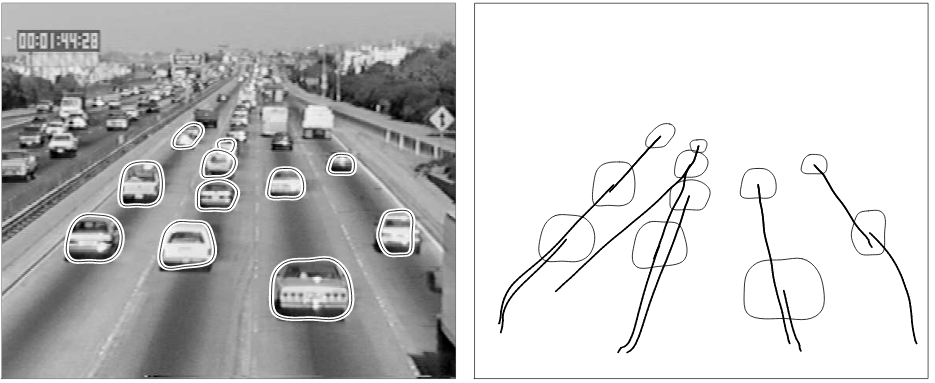
\includegraphics[width=0.9\textwidth]{figures/Introduccion/koller_weber_walik_oclusion.png}
		\caption{Ejemplo de detección y seguimiento de vehículos de~\cite{robust_multiple}}
		\label{fig.koller_weber_walik_oclusion}
		\end{center}
\end{figure}

G.D. Sullivan, K.D. Baker, A.D. Worral, C.I. Attwood, P.M. Remagnino~\cite{model_vehicle_detection} publicaron un sistema para la clasificación de vehículos empleando una combinación de plantillas en 1-D  y 2-D. Las plantillas 1-D se generaban sobre modelos de vehículos y las 2-D se empleaban para la verificación y aceptación de las hipótesis generadas en la primera fase del algoritmo de clasificación.Coifman et al.~\cite{areal_time} presentaron un algoritmo capaz de seguir un conjunto de características visuales de los vehículos ( en lugar del vehículo completo) con lo cual pretende ser más robusto ante oclusiones.

Las técnicas que se han ido publicando en las últimas décadas se presentan en dos escenarios (tráfico urbano y tráfico en autopistas). A continuación se explicará las situaciones que se encuentran en ambos escenarios.

\subsection{Visión computacional en tráfico urbano}\label{ap.vision_computacion_urbano}

En el análisis de tráfico urbano se pretende aplicar las técnicas de visión computacional en ciudades o entornos urbanos en general. En este caso la visión computacional se emplea para asegurar la aplicación de las normas de tráfico, para obtener información acerca del flujo de tráfico o para detectar posibles incidencias. El entorno urbano es un entorno muy complejo, pues existen demasiadas variables involucradas. Podemos tener peatones, ciclistas, edificios, señales de tráfico, árboles, otros vehículos, etc. Esto hace que sea más probable tener oclusiones en la imagen.

Una aplicación muy habitual en entornos urbanos es la detección de conductores que no respetan los semáforos en rojo. Para ello se   hace uso de cámaras que se encuentran conectadas a las luces del semáforo, y cada vez que éste se pone en rojo las cámaras se activan. Todo vehículo que sobrepasa la línea blanca una vez este el semáforo en rojo quedará fotografiado. Pero esto no siempre se tiene totalmente en cuenta, pues en muchas legislaciones es necesaria una prueba irrefutable de que el vehículo se ha saltado el semáforo. Esto se debe a que en muchos casos cuando un semáforo está en ambar los coches aceleran, corriendo el riesgo de pasar justo cuando el semáforo se ponga en rojo. Con el fin de evitar estos problemas, los sistemas han ido avanzando. Actualmente se graban toda la escena para poder asegurarse de si existe una infracción o no. La cámara se sitúa antes del semáforo para poder ver claramente a los vehículos infractores. Además se les ha incorporado un mecanismo para medir la velocidad de los vehículos que pasan y así poder ver si tienen alta probabilidad de saltarse los semáforos. Si superan cierta velocidad se considera que tienen una alta probabilidad de cometer una infracción y es entonces cuando la cámara se activa para grabarlo.
\begin{figure}[H]
  \begin{center}
    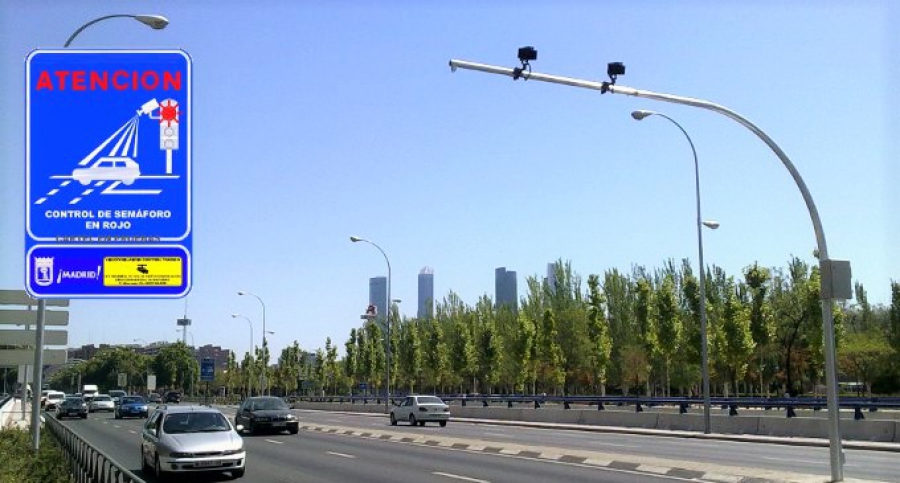
\includegraphics[width=0.6\textwidth]{figures/Introduccion/control_semaforo.jpg}
		\caption{Control de semáforos en rojo}
		\label{fig.control_semaforos}
		\end{center}
\end{figure}
En el tráfico interurbano una aplicación muy común es la detección de infracciones. Los centros de monitorización del tráfico disponen de muchas cámaras en las carreteras, pero el personal dedicado a revisar las imágenes que obtienen es bastante reducido, por lo que surge la necesidad de automatizar este proceso. A esta automatización de la detección de incidencias se le llama AID  y gracias a ella los trabajadores dedicados  a la monitorización del tráfico solo tienen que revisar las imágenes en las  cuales las cámaras han detectado una incidencia. El hecho de automatizar este proceso hace que el tiempo de intervención se vea reducido, pues son capaces de detectar las incidencias en menor tiempo, minimizando el tiempo de respuesta de los servicios sanitarios. Con esta información pueden actualizarse los paneles informativos, para avisar al resto de vehículos de la existencia de un accidente.

\begin{figure}[H]
  \begin{center}
    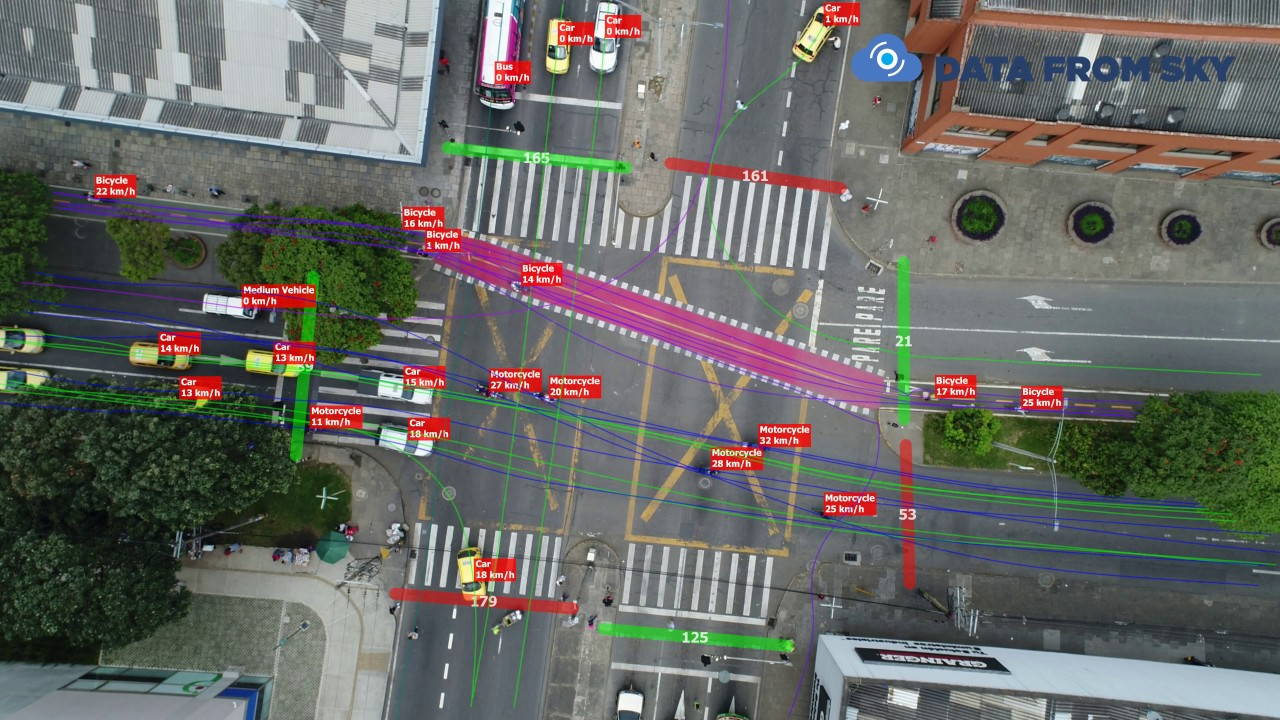
\includegraphics[width=0.75\textwidth]{figures/Introduccion/monitorizacion_trafico_urbano.jpg}
		\caption{Monitorización del tráfico urbano}
		\label{fig.monitorizacion_trafico_urbano}
		\end{center}
\end{figure}

Vermeulen~\cite{automatic_incident} para detectar incidentes combina la información visual con información obtenida por una cámara térmica. Con esto se consigue un sistema muy robustos ante las diferentes condiciones meteorológicas. Este sistema fue instalado en el puente de \textit{Rion} en Grecia. Chang et al~\cite{new_traffic_incident} presentó un sistema basado en la detección de matrículas para la identificación de incidencias. En este caso emplea la información del tiempo de viaje del vehículo para inferir incidencias en su trayectoria.

Otro tema en creciente desarrollo es el análisis del comportamiento de los vehículos en rotondas o bifurcaciones. A la hora de realizar modificaciones en las infraestructuras viales se realizan estudios acerca del flujo de vehículos que circulan por las redes de transporte, para ello es muy útil conocer el comportamiento de los vehículos. Nateghinia and Moradi~\cite{video_based_multiple} realizó un sistema capaz de seguir los vehículos en intersecciones y resolver el problema de las oclusiones. Para realizar las detecciones modelan cada píxel como una distribución gaussiana y lo combinan con el modelado dinámico de  textura. Shirazi and Morris~\cite{vision_based_turning} presentó un sistema un poco más evolucionado, pues a parte de seguir y contar los vehículos en cada intersección, era capaz de estimar la capacidad y el tiempo de espera en la intersección y reconstruir la trayectoria de los vehículos.

Finalmente, no hay que olvidarse de los túneles, los cuales juegan un papel importante dentro del tráfico urbano. De hecho en la M-30 en Madrid tenemos una longitud de 43 km de túneles, con el fin de reducir el flujo de tráfico sobre la superficie. Debido al gran uso de los túneles y la dificultad que existe para acceder a ellos en caso de accidentes, es necesario monitorizarlos. El uso de cámaras en los túneles hace que se pueda identificar la existencia de incidencias dentro de ellos, para actuar en el menor tiempo posible. En este caso una actuación rápida es esencial para evitar segundos accidentes o catástrofes en caso de incendios.

\begin{figure}[H]
  \begin{center}
    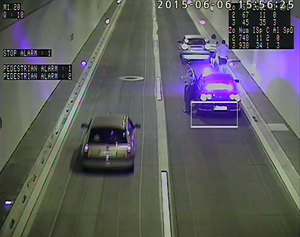
\includegraphics[width=0.6\textwidth]{figures/Introduccion/detection_tunel.png}
		\caption{Sistema de detección de incidencias en túnel}
		\label{fig.deteccion_tunel}
		\end{center}
\end{figure}

\subsection{Monitorización de autopistas basada en visión}

En este caso el análisis del tráfico se realiza en autopistas. Con ello se pretende obtener información acerca de la velocidad de los vehículos, el flujo de tráfico, la existencia de incidencias, etc. Este entorno es más sencillo que el comentado en el Apartado ~\ref{ap.vision_computacion_urbano}, ya que no hay que controlar tantas variables (peatones, edificios , etc), únicamente tendremos vehículos de diferentes tipos. 

\begin{figure}[H]
  \begin{center}
    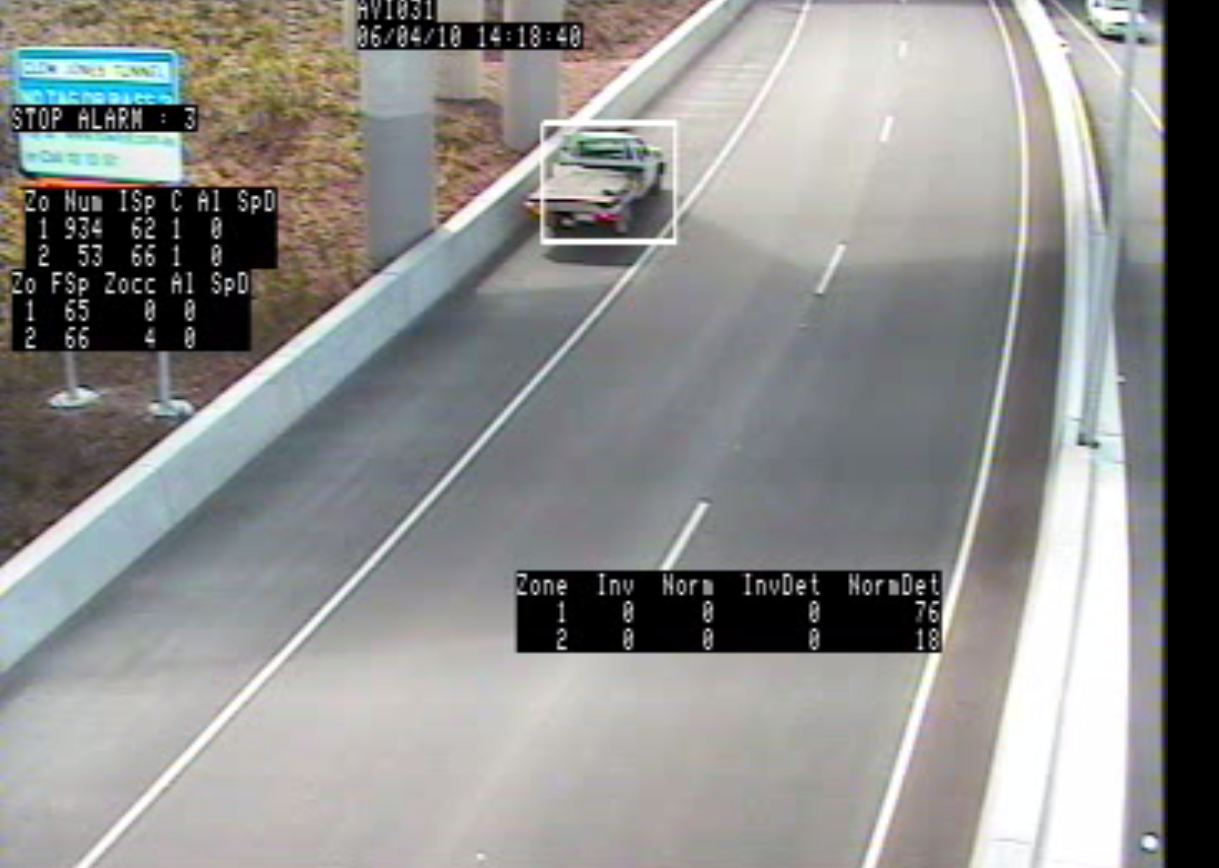
\includegraphics[width=0.6\textwidth]{figures/Introduccion/deteccion_autopistas.jpg}
		\caption{Sistema de detección de incidencias en autopistas}
		\label{fig.deteccion_autopistas}
		\end{center}
\end{figure}

La mayoría de los sistemas mencionados en el caso de entornos urbanos se emplean en las autopistas, ya que las incidencias que ocurren son similares. La principal diferencia entre ambos escenarios es la velocidad de los vehículos. En el tráfico urbano el límite de velocidad es bajo, pero en las autopistas es mucho más elevado y depende de cada país. En España el límite esta en 120km/h pero en Alemania la velocidad no está limitada. Esto se debe tener en cuenta a la hora de realizar el sistema de monitorización.

\section{Sistemas comerciales basados en visión}

Antiguamente la visión computacional solo se desarrollaba en el ámbito de la investigación pero actualmente se ha visto extendida hasta un ámbito comercial. Actualmente en el mercado hay numerosos sistemas basados en visión. Gracias a su reducido coste y su gran fiabilidad los sistemas basados en visión se han convertido en una alternativa perfecta a los sistemas clásicos de detección.

Desde los años 80 el empleo de la tecnología en los sistemas inteligentes de transporte ha ido creciendo. Esto se debe a que es un sector muy importante en los países en vías de desarrollo y en los países desarrollados. Algunas de las empresas que desarrollan este tipo de sistemas son: Flir (EEUU), Siemens (Alemania), Indra (España), Kapsch (Austria), Q-Free (Norguega), Thales (Francia), Sigtec(Austria).

Siemens es uno de los mayores proveedores de sistemas de control de tráfico a nivel mundial. Su familia de sistemas \textit{SitTraffic} ofrece un amplio abanico de funcionalidades.

FLIR es una empresa muy activa en este sector, pues ofrece sistemas con diversas funciones (detección automática de atascos, presencia de vehículos en las intersecciones, detección de peatones , etc).  Su sistema combina cámaras visuales y cámaras térmicas que le permiten regular las luces de tráfico. La serie de productos \textit{TrafiCam} realiza la detección y seguimiento de vehículos en intersecciones de forma automática; y permite posicionar y verificar con exactitud las zonas de detección de presencia de vehículos. Además este sistema mide la longitud de las colas que se forman en los atascos.

\begin{figure}[H]
  \begin{center}
    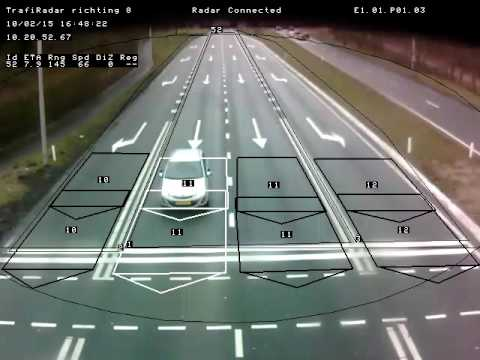
\includegraphics[width=0.6\textwidth]{figures/Introduccion/flir.jpg}
		\caption{Sistema \textit{TraffiCam} de FLIR}
		\label{fig.flir}
		\end{center}
\end{figure}

La empresa Morpho ha desarrollado un sistema basado en visión que pretende sustituir a los radares tradicionales. Se trata de su sistema \textit{Mesta Fusion}, el cual es capaz de detectar coches que circulen hasta a 300 km/h, puede controlar ocho carriles al mismo tiempo, supervisar 32 vehículos a la vez y discriminar entre ellos según sea un turismo, una moto, una furgoneta o un camión o autobús. Además es capaz de identificar casi cualquier acción indebida.  Todo eso lo hace un sistema perfecto en temas de monitorización de tráfico. Este sistema ya está operativo en Francia y Dubai.

\begin{figure}[H]
  \begin{center}
    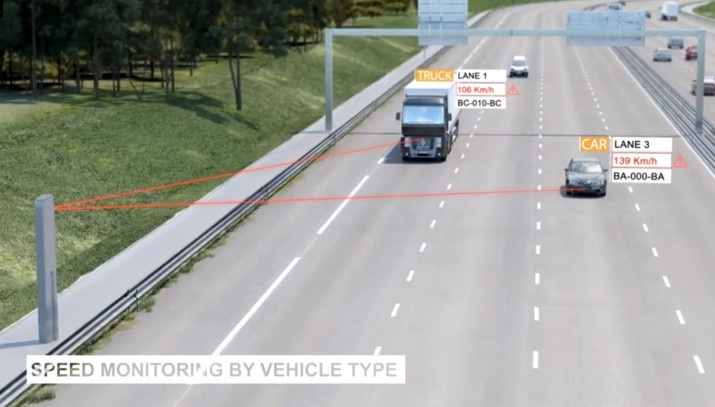
\includegraphics[width=0.6\textwidth]{figures/Introduccion/mesta_fusion.jpg}
		\caption{Sistema \textit{Mesta Fusion} de Morpho}
		\label{fig.mesta_fusion}
		\end{center}
\end{figure}

\section{Objetivos}

Este TFM se basa en la monitorización visual de transporte mediante el uso de una cámara. El objetivo principal de este proyecto es obtener un sistema capaz de detectar, clasificar y realizar un seguimiento de vehículos en tiempo real. Para ello se ha partido de un sistema inicial realizado por Redouane Kachach~\cite{redo_tesis} en su tesis doctoral. Dicho sistema se basa en técnicas clásicas. El objetivo es mejorar sus resultados con el uso de técnicas más actuales como el \textit{Deep Learning}.

Al hacer uso de \textit{Deep Learning} la detección y clasificación de vehículos van de la mano. En este trabajo se evaluaran diferentes  librerías relacionadas con el \textit{Deep Learning}, tales como \textit{TensorFlow}, \textit{Keras} y \textit{Darknet}, con el objetivo de emplear la que mejores resultados ofrezca.

La fase de clasificación debe identificar los vehículos en función de 7 categorías: Motocicletas, Coches, Furgonetas, Autobuses, Camiones Pequeños, Camiones y Camiones Cisterna. Esta es una mejora respecto al sistema del que se parte~\cite{redo_tesis}, pues en ese caso la clasificación se realizaba entre 5 tipos de vehículos. No existía la diferenciación entre los tres tipos de camiones, sino que eran una única catgoría.

En cuanto al seguimiento, el objetivo es tener la capacidad de realizar el tracking de cada vehículo durante todo el recorrido.

Para conseguir todos los objetivos mencionados es necesario recopilar una amplia base de datos que nos ofrezca datos de vehículos en diferentes condiciones meteorológicas, y con menor o mayor calidad de imagen, para tratar de conseguir un sistema lo más robusto posible.

Además el sistema debe cumplir los siguientes requisitos:
\begin{enumerate}
    \item El sistema tiene que emplear como sensor una cámara
    \item El sistema debe funcionar en tiempo real
    \item Las bases de datos que se han empleado durante el desarrollo del proyecto son de la parte trasera del vehículo, por lo que todos los videos que se evaluen tendrán esta característica. Para funcionar con otra orientación de la cámara tendríamos que emplear una base de datos mayor con diferentes orientaciones. Esto no se ha podido realizar debido a la falta e tiempo.
    \item  Los algoritmos están preparados para funcionar de día.
\end{enumerate}

Hay que decir que en la tesis de Redouane Kachach~\cite{redo_tesis} no se tuvieron en cuenta secuencias de video con diferentes tipos de condiciones meteorológicas, pero en este caso se pretende que el sistema sea capaz de funcionar con diferentes condiciones.  No obstante el sistema no se ha desarrollado para que sea capaz de funcionar por la noche.

\section{Estructura de la Memoria}

En el Capítulo~\ref{cap.introduccion} se comenta como la visión ha sido empleada en el campo de la monitorización del tráfico, y se realiza un breve repaso de la historia y evolución de esta disciplina.

El Capítulo~\ref{cap.estado} hace un repaso acerca de los trabajos científicos relacionados con la detección, clasificación y seguimiento de vehículos, los cuales sirven de referencia para nuestro estudio.
